\documentclass{standalone}
% translate with >> pdflatex -shell-escape <file>

% This file is an extract of the PGFPLOTS manual, copyright by Christian Feuersaenger.
% 
% Feel free to use it as long as you cite the pgfplots manual properly.
%
% See
%   http://pgfplots.sourceforge.net/pgfplots.pdf
% for the complete manual.
%
% Any required input files (for <plot table> or <plot file> or the table package) can be downloaded
% at
% http://www.ctan.org/tex-archive/graphics/pgf/contrib/pgfplots/doc/latex/
% and
% http://www.ctan.org/tex-archive/graphics/pgf/contrib/pgfplots/doc/latex/plotdata/

\usepackage{pgfplots}
\usepackage{pgfplotstable}
\pgfplotsset{compat=newest}

% The manual loads these libraries globally; the extracted standalone examples
% need them too. external/clickable/snakes are intentionally omitted.
\usetikzlibrary{
	arrows.meta,backgrounds,calc,decorations.footprints,decorations.markings,
	decorations.pathreplacing,fixedpointarithmetic,intersections,patterns,
	plotmarks,shapes.arrows,spy,through}
\usepgfplotslibrary{
	colorbrewer,colormaps,dateplot,fillbetween,groupplots,patchplots,polar,
	smithchart,statistics,ternary,units}

% Some colormap examples reuse this display style defined earlier in the manual.
\pgfplotsset{
	cycle from colormap manual style/.style={
		x=3cm,y=10pt,ytick=\empty,
		colorbar style={x=,y=,ytick=\empty},
		point meta min=0,point meta max=1,
		stack plots=y,
		y dir=reverse,colorbar style={y dir=reverse},
		every axis plot/.style={line width=2pt},
		legend entries={0,...,20},
		legend pos=outer north east,
	},
}

\pagestyle{empty}

\begin{document}
\pgfplotsset{
  colormap={whiteblue}{color=(blue) color=(white)},
  colormap={gb}{color=(green) color=(yellow)
      color=(brown)},
  of colormap/ocean height/.style={
      target pos={-12000,-10000,-6000,-5000,-3000,
          -1000,-750,-500,-250,-100,-50,0,10,100,
          200,500,1000,1100,1200,1500,2000,4000,
          6000,8000},
  },
  colormap={CM}{
      of colormap={
          whiteblue,
          ocean height,
          target pos max=0,
          sample for=const,
      },
      of colormap={
          gb,
          ocean height,
          target pos min=0.1,
          sample for=const,
      },
  },
}
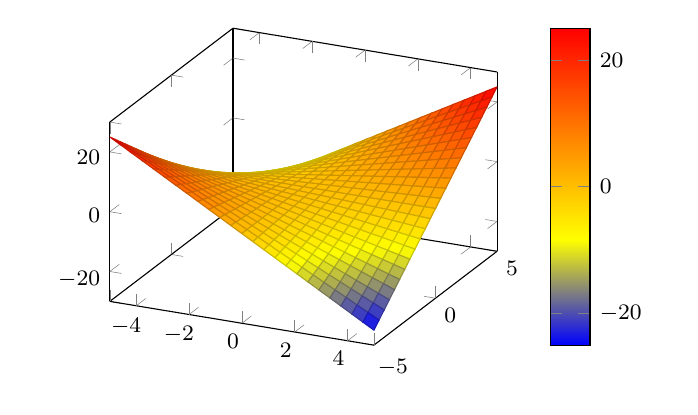
\begin{tikzpicture}
\begin{axis}[small,colorbar]
    \addplot3[surf] {x*y};
\end{axis}
\end{tikzpicture}
~
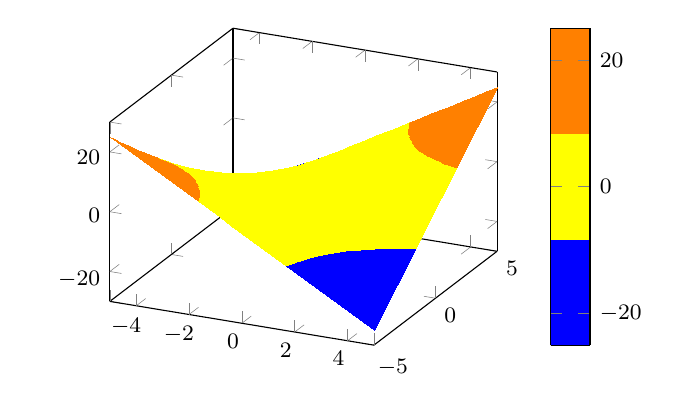
\begin{tikzpicture}
\begin{axis}[small,colorbar,
    colorbar style={colormap access=const}
]
    \addplot3[surf,shader=interp,colormap access=const] {x*y};
\end{axis}
\end{tikzpicture}
\end{document}
